\documentclass[border=0pt]{standalone}
\usepackage{amsmath}
\usepackage{tikz}
\usetikzlibrary{matrix, shapes.geometric, calc}
\begin{document}
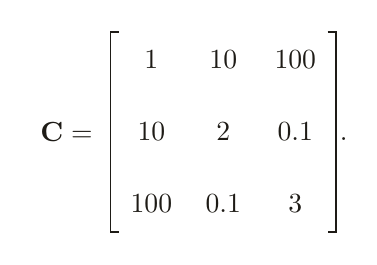
\begin{tikzpicture}
% Shared drawing of the symmetric matrix example in linear_algebra.qmd
% (@sec-special-matrices). \input by symmetric-matrix*.tex so the plain and
% annotated versions can never drift apart. Not built on its own: build.sh
% only compiles *.tex.
%
% Colours mirror the mfpa palette (_common.R / mfpa.scss).
\definecolor{mfpaink}{HTML}{1E1B16}
\definecolor{mfpateal}{HTML}{0F6E6E}
\definecolor{mfpared}{HTML}{B3261E}
\definecolor{mfpagreen}{HTML}{2E7D46}
\definecolor{mfpamuted}{HTML}{6B645A}
\tikzset{
  % Uniform ring around a single entry.
  entry ring/.style={draw=#1, ellipse, line width=1.1pt,
    minimum width=2.2em, minimum height=1.3em, inner sep=0pt},
  % Connector between mirrored entries.
  mirror link/.style={draw=#1, line width=0.9pt, dash pattern=on 2.5pt off 1.8pt},
}
\matrix (m) [matrix of math nodes, text=mfpaink, inner sep=0.35em,
    nodes={anchor=center, minimum height=1.3em, minimum width=2.2em, inner sep=0pt},
% Square grid (row pitch = column pitch = 2.6em), so the diagonal runs at
% 45 degrees and each mirror link is perpendicular to it, like a fold line.
    column sep=0.4em, row sep=1.3em] {
  1   & 10  & 100 \\
  10  & 2   & 0.1 \\
  100 & 0.1 & 3   \\
};
% Brackets drawn as plain strokes: TeX's extensible delimiters leave visible
% seams between their pieces once rasterized.
\draw[mfpaink, line width=0.55pt]
  ([xshift=0.3em]m.north west) -- (m.north west) -- (m.south west) -- ([xshift=0.3em]m.south west);
\draw[mfpaink, line width=0.55pt]
  ([xshift=-0.3em]m.north east) -- (m.north east) -- (m.south east) -- ([xshift=-0.3em]m.south east);
\node[text=mfpaink, anchor=east] at ([xshift=-0.3em]m.west) {$\mathbf{C} =$};
% Sentence-ending period (each image ends a sentence in the text), on the middle row's baseline as TeX would set it.
\node[text=mfpaink, anchor=base west, inner sep=0pt]
  at ([xshift=0.12em]m.east |- m-2-3.base) {.};
% Fixed bounding box shared by every version, so all PNGs have identical size
% and the matrix sits in the same place in each.
\path[use as bounding box] ([xshift=-3.0em, yshift=-0.15em]m.south west)
  rectangle ([xshift=0.45em, yshift=0.15em]m.north east);

\end{tikzpicture}
\end{document}
